\documentclass{article}
\usepackage[left=2cm, right=2cm, top=0cm]{geometry}
\usepackage{amsmath}
\usepackage{amssymb}
\usepackage{graphicx}
\usepackage{tikz}
\usepackage{enumitem}
\usepackage[margin=2cm]{caption}
\usepackage{hyperref}

\setlength\parindent{0pt}
\hypersetup{
    colorlinks,
    citecolor=green,
    filecolor=black,
    linkcolor=blue,
    urlcolor=blue
}

\begin{document}
\title{Assignment 3: Network Simulation}
\author{Jacob Puthipiroj}
% \date{}
\maketitle

\makeatletter
\newcommand{\mybox}{%
    \collectbox{%
        \setlength{\fboxsep}{1pt}%
        \fbox{\BOXCONTENT}%
    }%
}


\section*{Introduction}
In CS166, we explored models of social dynamics by using adaptive networks, and using in particular the NetworkX module available in Python. In this paper, I use the tools of network analysis to model the patterns of observed conformist and nonconformist ('hipster') modes of behavior. 

\section*{Model Assumptions}
The model has two core assumptions:
\begin{enumerate}
\item In the most basic model, the population is split into anticonformists ('hipsters'), who take their decisions in opposition to the majority, and the conforomists ('mainstreams', 'normies') who follow the majority.  
\item The lag time needed by each individual to detect and react to the changes of states is hetergeneously distributed. In the default specified in the model, the log-normal distribution was chosen to roughly follow the 'technical adoption cycle' - a few individuals will respond quickly to a perceived trend in the public sphere, a large majority will take a middle amount of time, and a small percentage will take very long time. 
\end{enumerate}
A further assumption worth mentioning, though not specific to the the hipster simulation, is the heterogeneous interactions between agents. Empirically, some individuals in the real world naturally have more influence than others: trend makers, bloggers, pundits, etc. The degree distribution of follows a power law. We implement the hipster simulation on both a watts-strogatz graph, as well as a barabasi-albert graph to encompass these observed behaviors, though we have not tried a graph that simultaneously follows a power-law degree distribution, as well as generates local clustering.\\

The probability of hipsters is fixed, and distributed heterogeneously across the population. However, the way in which an individual reacts with the environment is idiosyncratic. The system can also be described as stochastic, since individuals are randomly chosen to react to the environment, and reaction also follows a bernoulli distribution. As a result the state of any given individual follows a Markov jump process. To see, this, consider a network with 2 nodes and 1 edge.

\section*{Local Analysis}
There are 3 possible combinations of 2-node simulations:
\begin{enumerate}
\item \textbf{2 Conformists:} In this case, it is clear that if both nodes start off with the same opinion, then both opinions will continue to converge regardless of any possible differing lag times. Even if the two nodes are initialized differently, one node will immediately snap to the opinion of the other, and the two opinions will continue to converge indefinitely. 
\item \textbf{2 Hipsters:} If both nodes start off with differing opinions, then the two nodes will converge at a state of disagreement. Interestingly, the state of opposition seems to be the analogous to the state of total convergence for the 2 conformists. If both nodes are initialized similarly, then opinions will oscillate to maintain the state of divergence. Even if both nodes have the same lag time, convergence will not happen because node opinions are updated asynchronously. 
\item \textbf{1 Conformist, 1 Hipster:} In this case, the opinions of both nodes will rapidly oscillate back and forth indefinitely. As the conformist node attempts to copy the opinion of the hipster node, the latter will attempt to deviate from the former.   
\end{enumerate}

\newgeometry{left=2cm, right=2cm}
\begin{figure*}[h]
\centering
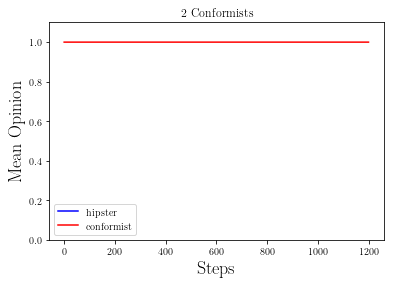
\includegraphics[scale = 0.6]{2conformists.png}
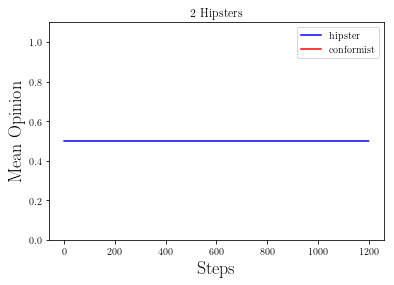
\includegraphics[scale = 0.6]{2hipsters.png}
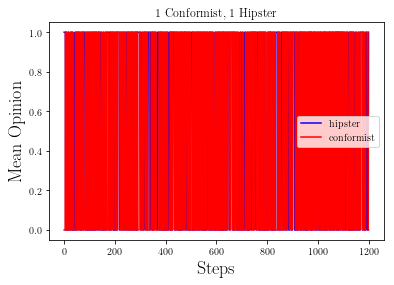
\includegraphics[scale = 0.6]{1ofeach.png}
\caption{The toy model involving 2 hipsters are remarkably similar, though notice the different scales - the 2 conformists converge at absolute agreement, while the 2 hipsters converge at absolute disagreement. The model involving both 1 conformist and 1 hipster however shows extreme oscillatory behavior.}
\end{figure*}




\section*{Implementation and Simulation Analysis}
The link to the full code for this section is available in the appendix. \\

The Hipster simulation was tried on both a Watts-Strogatz graph, with a corresponding Barabasi-Albert graph with an equivalent number of nodes and edges. 
\newpage

\newgeometry{left=2cm, right=2cm}
\begin{figure*}[h!]
\centering
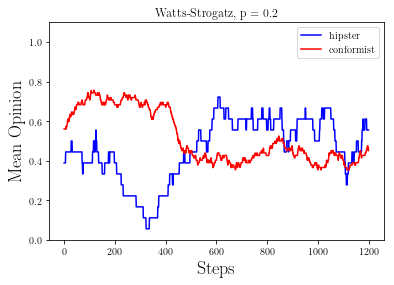
\includegraphics[scale = 0.6]{ws1.png}
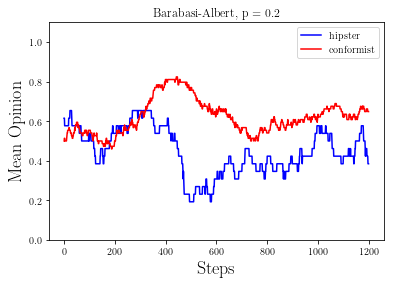
\includegraphics[scale = 0.6]{ba1.png}
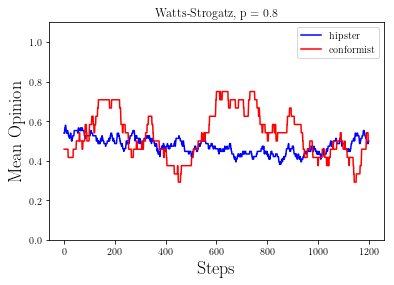
\includegraphics[scale = 0.6]{ws4.png}
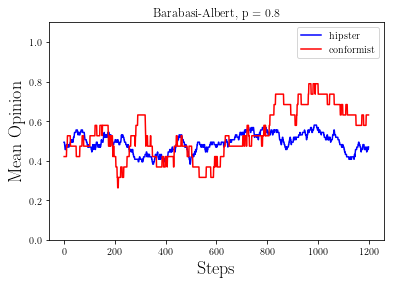
\includegraphics[scale = 0.6]{ba4.png}

\caption{In both the Watts-Strogatz graph as well as the corresponding Barabasi-Albert graphs, it is clear that the behavior of the hipsters and conformists seem to usually trend in different directions. This is clearest in the top-right graph, where it is clear that while the mean conformist opinion tends upwards, the hipsters counteract in turn by drastically switching their opinions at around the 400-step mark. Another observation is that in the bottom two graphs, where the hipsters form the majority opinion, the line seems to self-regulate at 0.5. In general, the red conformist line follows much wilder swings than the blue hipster line.}
\end{figure*}

Because of the bare-bones nature of the model, the scope of generalizability of this model is rather limited. For example, the formation of new relationships, as well as the strength of relationships were not at all considered, and would be an interesting and highly conducive direction of future work. The aim of this paper is to model the paradoxical behavior of hipster communities, where hipsters seem to adopt the same behaviors despite wanting to avoid being labelled, was observed only in networks where they comprised the minority - most clearly in the Watts-Strogatz graph, where the hipsters seem to unidirectionally alter their opinion to contrast against the mainstream opinion of the public, and then immediately gain popularity as fewer conformists adopt the belief. \\




\newpage
\section*{Appendix}


\subsection*{MultiLane Traffic Flow}
The code used in this section is available \href{https://github.com/thetruejacob/CS166/blob/master/Rickert%20Model.ipynb}{here}.



\end{document}